\section{Code Size}
\label{sec:res:code-size}

This section looks at the size of the compiled binaries for three {\rust} programs.
These programs are the two projects, {\tracker} and {\cg}, and a Minimal Main program.
A comparison between functionally equivalent programs in {\C} and {\rust} are provided.

Code size is an important factor in an embedded system.
The systems are more restricted than conventional systems, especially when it comes to storage.
For the EFM32 line of microcontrollers the code is stored in flash memory.
In \autoref{sec:back:hw}, we showed that the flash memory in the EFM32 family of microcontrollers ranges from 4KB to 1MB.
As \autoref{sec:before-main} explains, the flash memory should not only contain the program code but also the constant data defined in the program.
This limits the code size even further.

Another concern that makes code size a priority in embedded system is price.
When putting embedded systems into production, the volume of microprocessors are usually large.
Moreover, as the size of the flash correlates with the price of the microprocessors, being able to choose a smaller version can save large amounts of money.

Each program was compiled with optimization levels O0, O1, O2, and O3, and the O0 level was compiled both with and without debugging symbols.
Compiling executable programs results in an {\elf} binary file.
The size was calculated by executing the \prog{arm-none-eabi-size} program.

\subsection{Measuring Size}
\label{sec:measure-size}

The \prog{arm-none-eabi-size} program accepts an {\elf} binary as argument.
The program then reads the file and reports the size of the \elfsec{.text}, \elfsec{.data} and \elfsec{.bss} segments described in \autoref{sec:back:elf}.

\subsection{Parameters}
\label{sec:size:params}
The various files were compiled by setting the compiler optimization flags in the \file{Cargo.toml} file.
The parameters used are shown in \autoref{tab:size:params} with their effects.

\begin{table}[H]
  \centering
  \begin{tabular}{l|l|l}

    \textbf{Parameter} & \textbf{Values} & \textbf{Effect} \\
    \hline
    \flag{debug} & true, false & Sets the \textbf{-g} flag on the compilers  \\
    \flag{debug-assertions} & true, false & A way to remove assertion statements \\
    \flag{opt-level} & 0, 1, 2, 3 & Sets the optimization flag on the compilers \\
    \flag{lto} & true, false & Sets the \gls{lto} flag on the linker \\
    \hline
  \end{tabular}
  \caption{\file{Cargo.toml} parameters and their effects}
  \label{tab:size:params}
\end{table}

Each program in this section is compiled with 6 different settings, as given by \autoref{tab:size:settings}.
\begin{table}[H]
  \centering
  \begin{tabular}{l|l|l|l|l|l|l}
    \textbf{Parameter} & \textbf{1} & \textbf{2} & \textbf{3} & \textbf{4} & \textbf{5} & \textbf{6} \\
    \hline
    \flag{debug}            & true  & false & false & false & false & false \\
    \flag{debug-assertions} & true  & false & false & false & false & false \\
    \flag{opt-level}        & 0     & 0     & 1     & 2     & 3     & 3     \\
    \flag{lto}              & false & true  & true  & true  & true  & true  \\
    (c code Os)      & false & false & false & false & false & true \\
    \hline
  \end{tabular}
  \caption{Compilation settings}
  \label{tab:size:settings}
\end{table}

For each of the optimization levels the underlying {\C} sources are compiled at the same level as the {\rust} code.
Notice that for the 6th optimization setting, the underlying {\C} sources are compiled with the Os flag, while the {\rust} sources are compiled at O3.

\subsection{Binary Sizes}

This subsection considers the code size of programs.
Functionally equivalent versions were written in both {\rust} and {\C}, and here we compare the size of the binaries produced at each optimization level presented in \autoref{tab:size:settings}.
\autoref{fig:size:bin:large} presents the sizes of the generated binaries for the two projects described in \autoref{sec:impl:projects}.

\begin{figure}[H]
  \begin{center}
    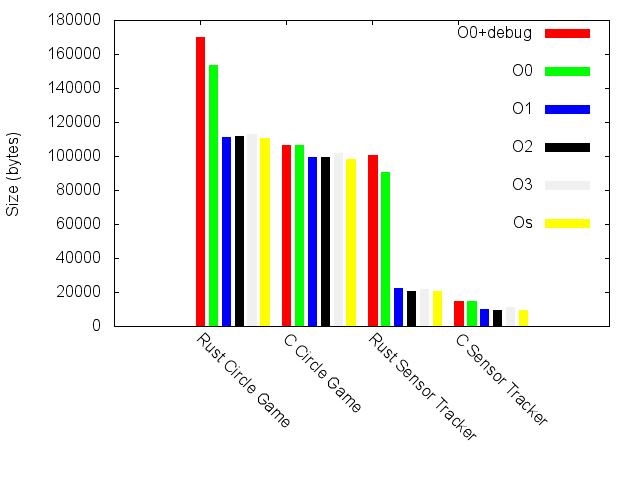
\includegraphics[scale=0.5]{results/plots/size/bin/large/size.png}
  \end{center}
  \caption{Code size for project binaries}
  \label{fig:size:bin:large}
\end{figure}


We see here that the largest variation is between unoptimized and optimized {\rust} code.
The sizes varies less for the other optimization levels.
Notice that the O2 level provides a smaller binary than the O3 version, and that the Os level consistently produces the smallest binaries.

\autoref{fig:size:bin:small} shows the code size of a minimal program to boot the {\gecko}.
Both implementations contains only an infinite loop, and we evaluate these to examine the overhead of the languages.

\begin{figure}[H]
  \begin{center}
    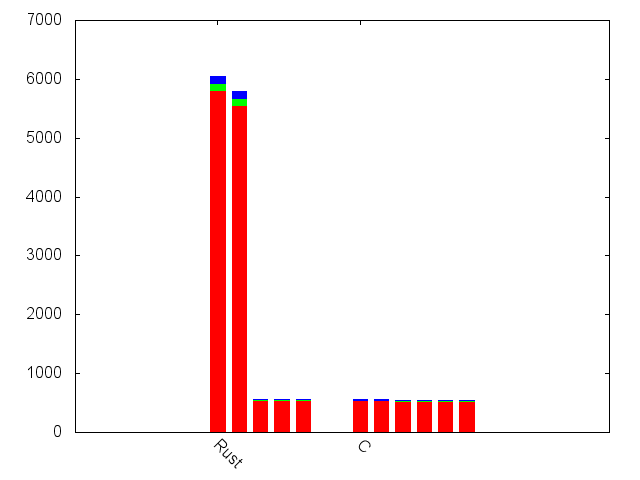
\includegraphics[scale=0.5]{results/plots/size/bin/small/size.png}
  \end{center}
  \caption{Code size for minimal program}
  \label{fig:size:bin:small}
\end{figure}

As explained in \autoref{sec:impl:booting}, {\rust} does not require any additional initialization or setup compared to {\C}.
This is evident in \autoref{fig:size:bin:small}, where the binaries are the same size when optimizations have been applied.
The debug and unoptimized {\rust} build is 10x larger than the optimized version.

To explain this increase in size, we look at the \emph{zero-cost abstractions} provided by {\rust}.
Some of these abstractions are built with numerous function invocations to handle complex use-patterns.
To be able to debug these abstractions, it is important that the compiler keeps all these functions in the unoptimized binary.
When one of these abstractions are used in the code (e.g. a \code{for} loop) most of these funtions becomes superfluous, and be inlined after applying \gls{dce}.

\autoref{tab:size:c-vs-rust} compares the size of the smallest {\C} and {\rust} binaries for each of the evaluated programs.
The number reported is generated by dividing the size of the {\rust} binary by the size of the {\C} binary, giving the factor of which the {\rust} version is larger than the {\C} version.

\begin{table}[H]
  \centering
  \begin{tabular}{c|c}

    \textbf{Program} & \textbf{Relative Size} \\

    {\cg} & 1.22x \\
    {\tracker} & 2.20x \\
    \texttt{MinimalMain}     & 1.00x \\
    \hline
  \end{tabular}
  \caption{{\rust} code size relative to {\C}}
  \label{tab:size:c-vs-rust}
\end{table}

We see from \autoref{tab:size:c-vs-rust} that the {\cg} binary comes quite close to the {\C} binaries in size.
The {\rust} \texttt{MinimalMain} shows no increase over the {\C} binary.
In \autoref{tab:size:breakdown}, we break down the size of the optimized binary of the {\tracker} to see which portions of the {\rust} code makes the binary size increase.

\begin{table}[H]
  \centering
  \begin{tabular}{l|r|r|l}
    \textbf{Section}      & \textbf{C (B)} & \textbf{Rust (B)} & \textbf{Relative} \\
    \hline
    \textbf{app}          & 1776 & 3964 & 2.23x \\
    \textbf{binding}      & 0    & 184  & N/A  \\
    \textbf{emlib}        & 4348 & 4376 & 1.01x \\
    \textbf{REL}          & 0    & 3516 & N/A  \\
    \textbf{newlib}       & 2372 & 792  & 0.33x \\
    \textbf{system}       & 460  & 896  & 1.95x \\
    \textbf{unwind}       & 0    & 3820 & N/A  \\
    \hline
  \end{tabular}
  \caption{Breakdown of binary sizes for the {\tracker} application}
  \label{tab:size:breakdown}
\end{table}

In \autoref{tab:size:breakdown}, we see that there are three major non-constant contributors\footnote{The \textbf{system} section increased with $\sim$2x, but this section will remain constant as the complexity of the application increases.} to the increased size for the {\rust} binary:

\begin{itemize}
\item The application
\item Rust Embedded Library
\item {\rust} expection mechanism (unwind)
\end{itemize}

We see that the \lib{newlib} implementation is reduced in the {\rust} binary.
This is due to the \gls{rel} library implementing some of the same functionality as \lib{newlib}.
Thus, this part of \lib{newlib} is not included.

%\subsection{Discussion}

%This section has shown that the code size of all {\rust} binaries are larger than their {\C} counterparts.
%The optimized {\rust} builds does come close to {\C} builds with being 1.94x larger on average, while the debug builds are far bigger, 6.88x on average.

%The test hardware used to produce the results given here is the EFM32GGF1024, as mentioned in \autoref{sec:back:hw}.
%This chip has 1MB for storing the code and therefore running the debug builds which maxed out at ~176KB, was not a problem.

%Considering the Minimal Main debug binary presented in \autoref{fig:size:bin:small} and comparing to the chips with lower specifications in the EFM32 family (\autoref{tab:efm32-family}), we see that a debug build can not be executed at small versions of the Zero and Tiny Gecko.
%Looking at the {\tracker} application, even the heavily optimized version of the {\rust} build can not run on the largest version of the either the Zero or Tiny Gecko.

%Reading the results presented here should take in mind that the comparisons are made between a mature production proven compiler \textbf{gcc} and a pre/close to 1.0 compiler \textbf{rustc}.
%The design objectives for the 1.0 version of {\rust} as outlined in \autoref{sec:rust:roadmap} has been on stabilizing the language APIs and features.
%This indicates that non-breaking changes like compiler optimizations both for compiler speed and binary code sizes not has been a priority leading up to the 1.0 release.
